%%%%%%%%%%%%%%%%%%%%%%%%%%%%%%%%%%%%%%%%%
%%% WP01
%%%%%%%%%%%%%%%%%%%%%%%%%%%%%%%%%%%%%%%%%

\tsubsubsection{WP3 - Access to RI for Accelerators}

%%%%%%%%%%%%%%%%%%%%%%%%%%%%%%%%%%%%%%%%%
%%% Section content, please change!
%%%%%%%%%%%%%%%%%%%%%%%%%%%%%%%%%%%%%%%%%

\subsubsection*{Overview and Goals}

% --- Data taken from Grant Agreement page 59

\begin{table}[H]
    \renewcommand{\arraystretch}{1.50}		
    \footnotesize   
    \begin{tabular}{*{3}{|p{0.10\textwidth}}|l|}
        \hline
        \rowcolor{mygray} \multicolumn{4}{|c|}{\textit{\color{white}Work Package Summary}} \\
        \hline
        \rowcolor{mylightergray} \textit{WP No.} & \cellcolor{white} 3 & \textit{Title of WP} & \cellcolor{white} (TA2): Access to Research Infrastructures for Accelerator R\&D \\
        \hline
        \rowcolor{mylightergray} \textit{Start} & \cellcolor{white} M1 & \textit{End} & \cellcolor{white} M48 \\
        \hline
        \rowcolor{mylightergray} \multicolumn{4}{|p{0.978\textwidth}|}{\textit{Participating Organisations}} \\
        \hline
        \multicolumn{4}{|p{0.978\textwidth}|}{
            \hspace*{-0.75cm} 
            \begin{minipage}[t]{\textwidth}
    			\begin{itemize}
    			    \item WP Leader: 3 CERN
    				\item Participants: CERN, UU, CEA, CNRS, KIT, INFN, INCT, UKRI
    			\end{itemize} 
    			\vspace*{0.10em}
			\end{minipage}
        } \\
        \hline
    \end{tabular}
    \vspace{0.5em}\vfill
    \begin{tabular}{|p{0.978\textwidth}|}
        \hline
        \rowcolor{mylightergray} \textit{Goals} \\
        \hline
        \rowcolor{white} 
        \hspace*{-0.75cm} 
        \begin{minipage}[t]{\textwidth}
        {\leftskip=15pt
        The work-package groups leading Research Infrastructures (RIs) offering trans-national access related to accelerator
R\&D across Europe.
    		\begin{itemize}
    		    \item Task 3.1 – (TA) for Material testing, lead by CERN

    			\item Task 3.2 – (TA) to Technology infrastructures, lead by CEA

			    \item Task 3.3 – (TA) to Electron and plasma beams, lead by UKRI-STFC
                    \item Task 3.4 – (TA) for TA related to Applications, lead by INCT
    		\end{itemize} 
    		\vspace*{0.10em}
        }
	\end{minipage}        
        \\
        \hline
    \end{tabular}
    \vspace{0.5em}\vfill
    \resizebox{\textwidth}{!}{%
    \begin{tabular}{|l|*{8}{>{\centering\arraybackslash}p{0.084\textwidth}|}}
        \hline    
        \rowcolor{mylightergray} \textit{Participant number} & \textit{1} & \textit{2} & \textit{3} & \textit{4} & \textit{5} & \textit{6} & \textit{7} & \textit{8} \\
        \hline
        \rowcolor{white} \cellcolor{mylightergray}\textit{Participant short name} & CERN & UU & CEA & KIT
                                                                                  & INFN & INCT & UKRI & CNRS \\
        \hline
        \rowcolor{white} \cellcolor{mylightergray}\textit{PM per participant~\footnotemark} & 16.5 & 20 & 20 & - & 21 & 16 & 6 & 13\\
        \hline        
    \end{tabular}
    }
\end{table}
\footnotetext{the PM figures correspond to the full duration of the project.}

\subsubsection*{Status}

\begin{figure}[!h]
    \centering
    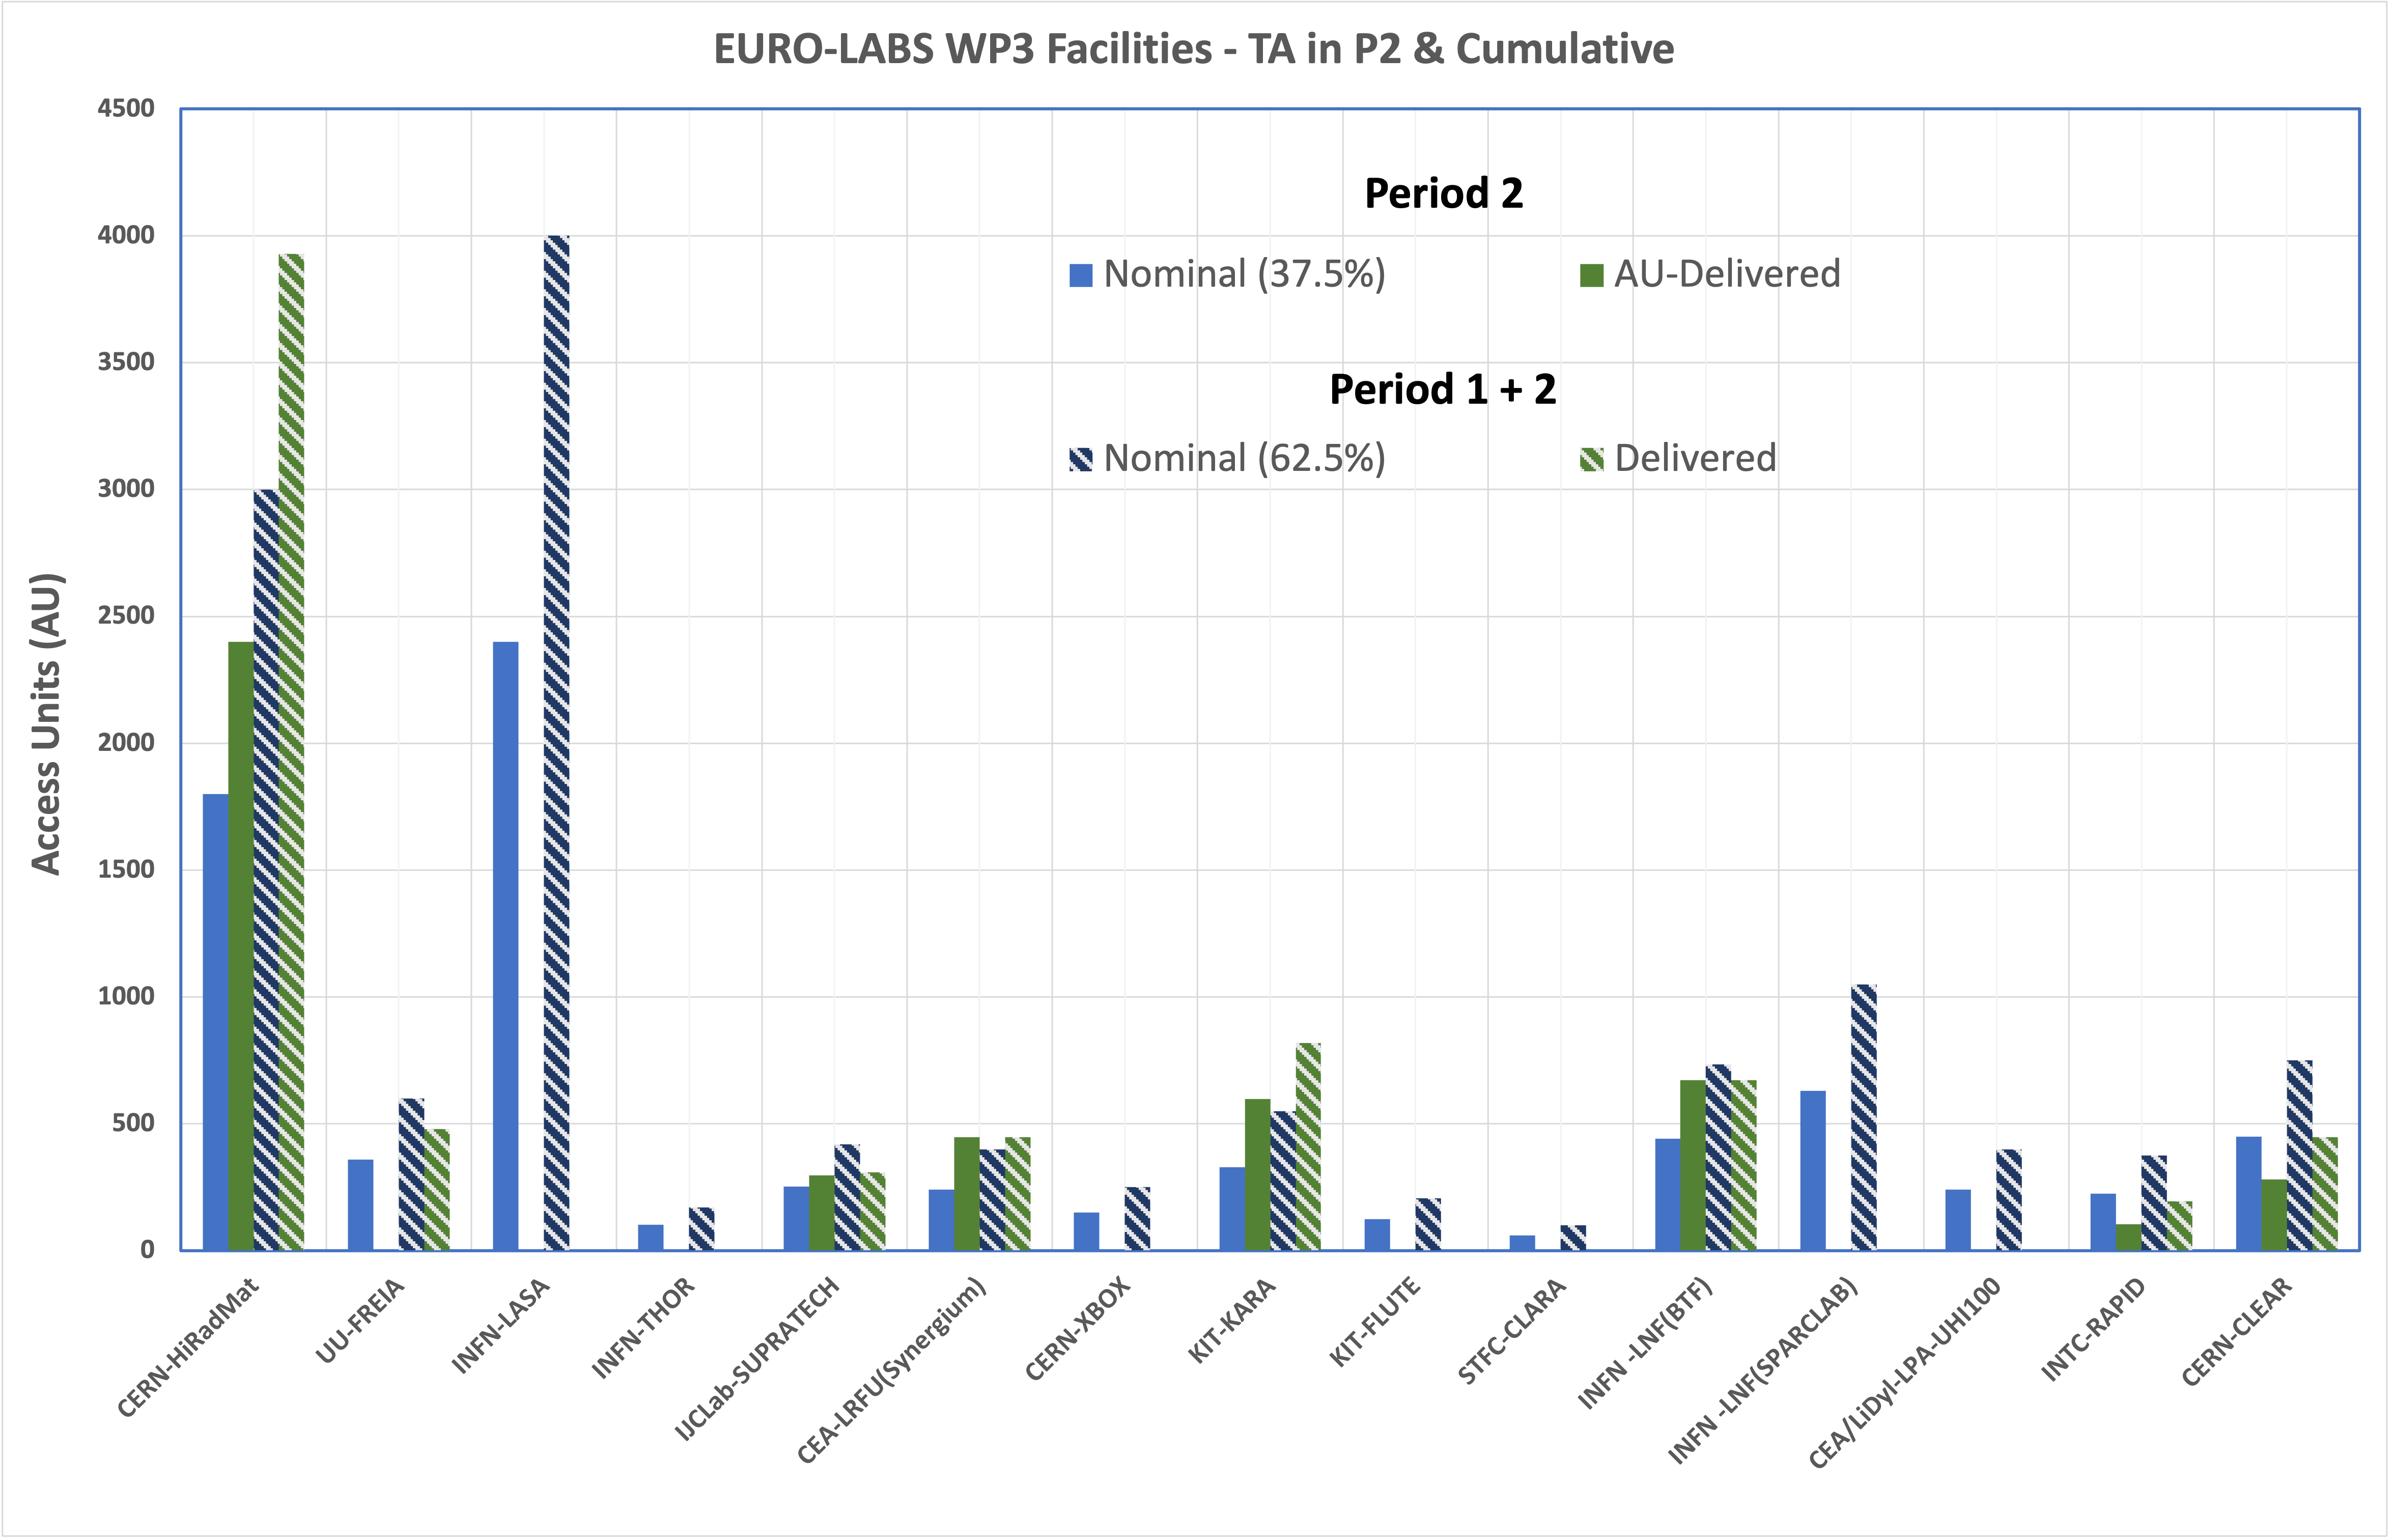
\includegraphics[width=0.98\linewidth]{graphics/WP3-TAstatistics.png}
    \caption{Distribution of AU (typically hours of beam time) delivered in P2 and cumulative for the full duration of the project. The values in the Nominal column represent the fraction of AU for the 18 months of the P2 (37.5\%) or to the 30 months for P1 and P2 (62.5\%) assuming a linear profile.}
    \label{fig:wpe-taunits}
\end{figure}
Over the 18 months covered in P2, the WP3 TA facilities have generally been rather successful in achieving the delivery of transnational access to users. Overall 4799 AU were delivered during P2, representing 84\% of an assumed linear fraction for these 18 months of the AU promised in the GA. The cumulative total for P1 and P2 raises to 7297 AU delivered, corresponding to 56\% of the total number of planed AU for the duration of hte project. This may sound small, however factoring out the facilities where technical or administrative hurdles impacted their capacity to deliver AU, this raises to 78\% which is well within expectations for this stage of the project. The distribution of the AU delivered per TA faciliy is shown in Fig~\ref{fig:wpe-taunits}.

The imbalance between facilities that have exceeded expectations in delivering transnational access (TA) units and those that have experienced inactivity has been thoroughly discussed during the Task and WP meetings. It was agreed that progress will continue to be closely monitored over the coming months. In parallel, a plan has been developed involving a reshuffling of project resources between facilities. This strategy aims to provide additional support to high-demand facilities and ensure the smooth operation of TA delivery for the benefit of the Users.

Beyond transnational access, steady progress has been achieved in the service improvements planned for eight facilities. In most cases, the implementation is ongoing, with the goal of completing these improvements and making them fully operational for the Users before the end of the project.

% \todo{Briefly explain the status of the WP.}

\subsubsection*{Progress per Task}

\subparagraph{Task 3.1 Material Testing Facilities} \mbox{}

This task includes only the HiRadMat Facility at CERN. 

\subparagraph{HiRadMat at CERN}

HiRadmat has had great progress in the last reference period concerning EURO-LABS. The facility remains in extremely high demand from the international community, involving both EU and overseas teams that are performing experiments. A total of 3928 AUs have been spend (from the total requested 4800). The percentage of AUs spent vs the available AUs and the evolution since the start of the project is shown in Figure~\ref{fig:wp3-hrmt-stat}. With the updated schedule of CERN, the facility will remain operational in 2026, the last year of EURO-LABS, and could welcome additional TA requests, also in view of the long shutdown 2026-2029. 
\begin{figure}[!h]
    \centering
    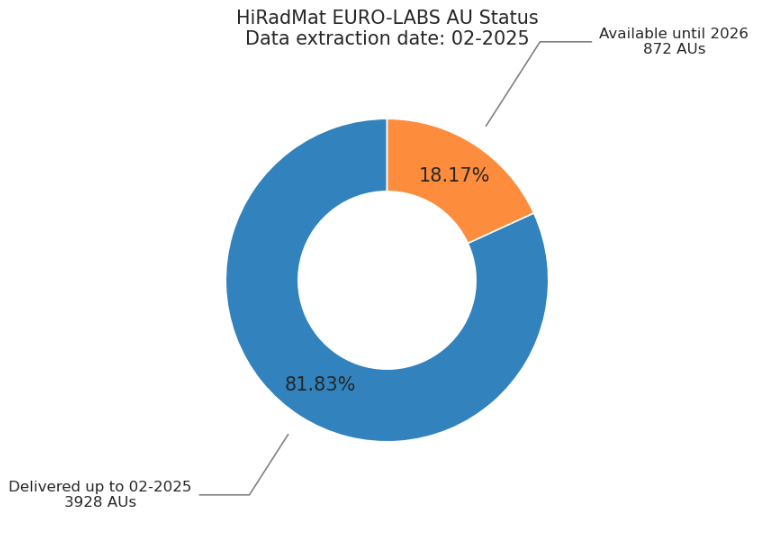
\includegraphics[width=0.48\linewidth]{graphics/stat_pie_hiradmat.png}
    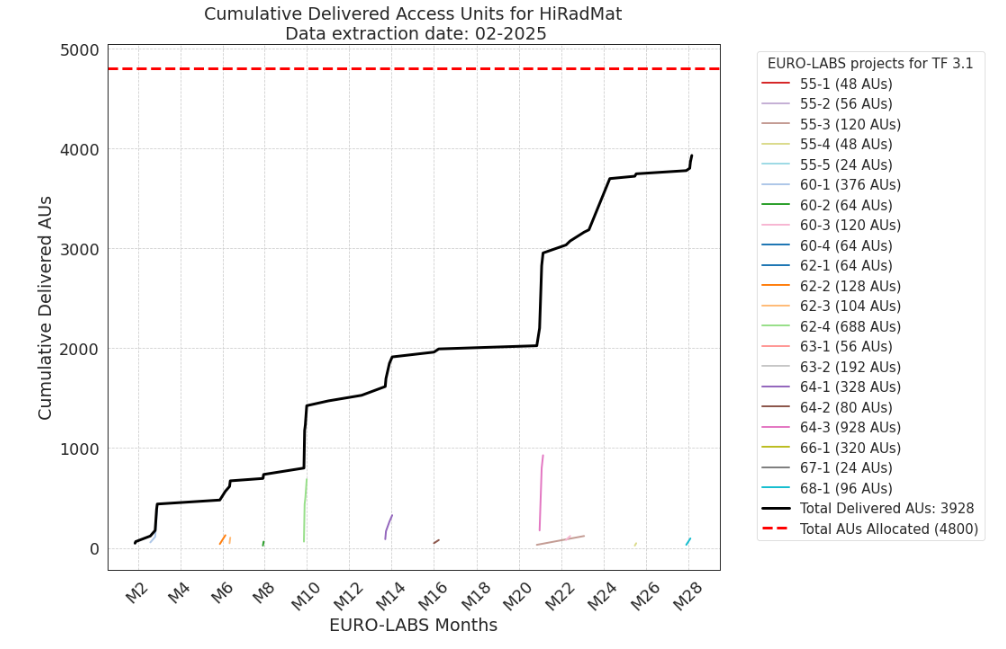
\includegraphics[width=0.48\linewidth]{graphics/overall_evolution_hiradmat.png}
    % \captionsetup{justification=centering}
    \caption{Access Units spent (left) and evolution in time (right) in HiRadMat to the end of P2.}
    \label{fig:wp3-hrmt-stat}
\end{figure}

% The evolution of the spent access units overall, and only for the RP2 is shown in Figures~\ref{fig:overall_evolution_hiradmat} and~\ref{fig:RP2_evolution_hiradmat}.
%\begin{figure}[!h]
%    \centering
%    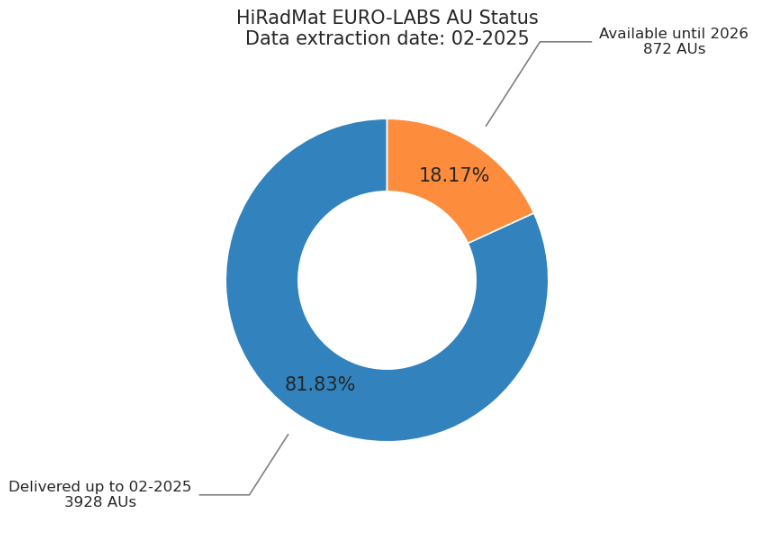
\includegraphics[width=0.75\linewidth]{graphics/stat_pie_hiradmat.png}
%    \caption{Access Units spent in HiRadMat in all reference periods. A total of 4800 AUs were allocated to the facility ; 3696 AUs have been already spent in this second reference period, and 232 AUs have been spent after September 2024 and until today (Feb. 2025). }
%    \label{fig:stat_pie_hiradmat}
%\end{figure}

Figure~\ref{fig:gender_distr_hiradmat} shows the gender and age distribution of the funded users in HiRadMat. 
\begin{figure}[!h]
    \centering
    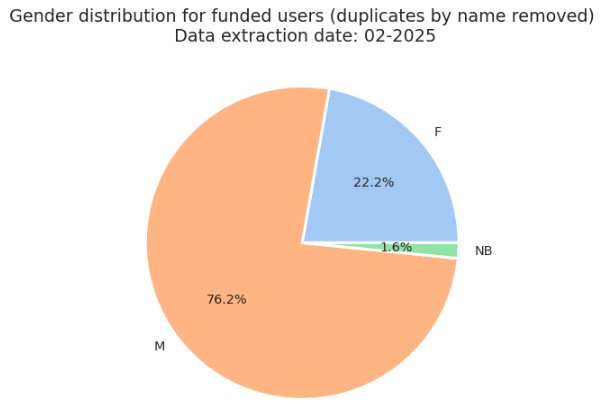
\includegraphics[width=0.48\linewidth]{graphics/gender_distr_hiradmat.png}
    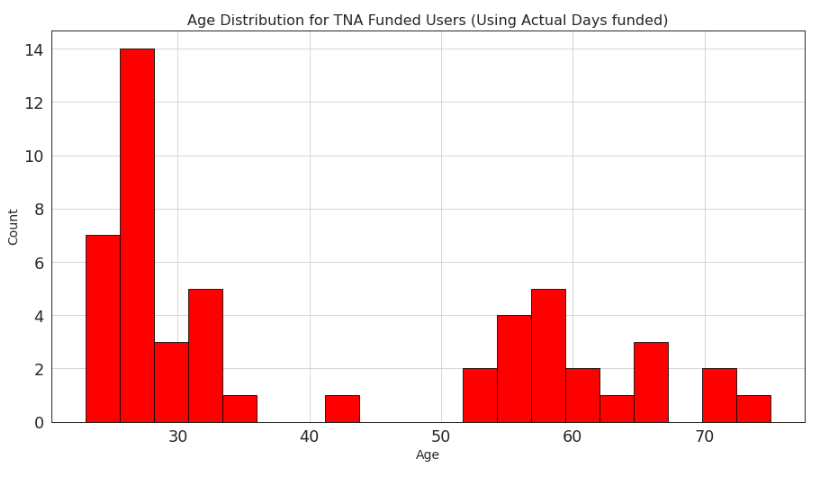
\includegraphics[width=0.48\linewidth]{graphics/age_distr_hiradmat.png}
    % \captionsetup{justification=centering}
    \caption{Gender(left) and age (right) distribution of TA funded users in HiRadMat.}
    \label{fig:gender_distr_hiradmat}
\end{figure}
The age distribution reflects the effort made within the USP to promote graduates and young researchers in the early stages of their careers. At the same time, the presence of senior researchers in the preparatory, data-taking and experimental phases is absolutely necessary for the success of the experiments and the transfer of knowledge. 

%For the funded users, the gender distribution is shown also in Figure~\ref{fig:gender_distr_hiradmat}, removing the duplicates by name. 
% is indicating that as per the instructions for TA, the user selection panel has approved mostly undergraduate and postgraduate students, at the early stages of their careers and fewer senior researchers (professors and tenured researchers). However, specifically at HiRadMat, the presence of the 
%The age distribution for the funded users is shown in Figure~\ref{fig:age_distr_hiradmat}.
%\begin{figure}[!h]
%    \centering
%    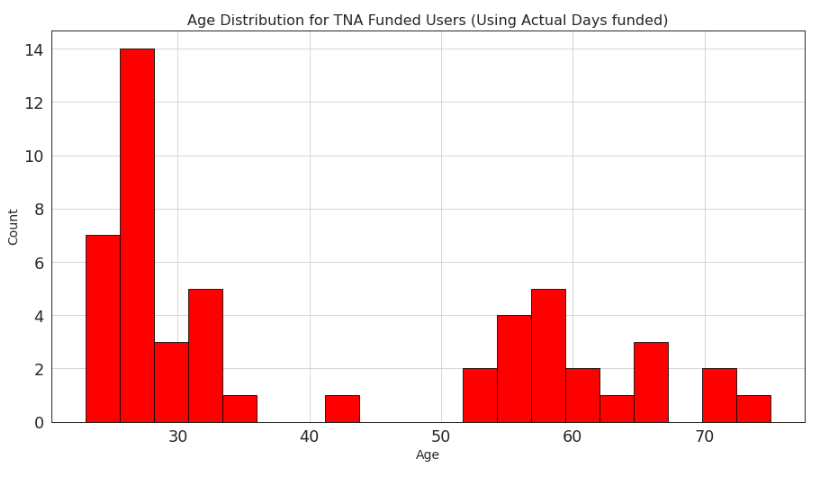
\includegraphics[width=0.75\linewidth]{graphics/age_distr_hiradmat.png}
%    \caption{Age distribution of funded users in Task 3.1 (HiRadMat). The majority of the supported users is at the early stages of their career, while a few senior researchers or recognized scientists at their field have been also necessary during the preparatory or the post-irradiation phases.}
%    \label{fig:age_distr_hiradmat}
%\end{figure}
%\begin{figure}[!h]
%    \centering
%    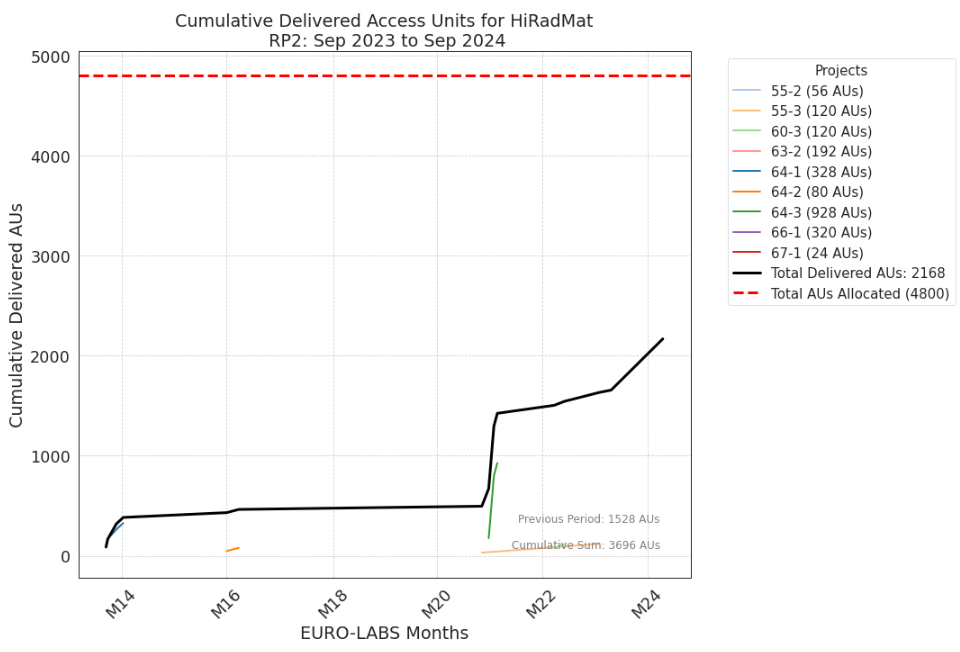
\includegraphics[width=0.9\linewidth]{graphics/RP2_evolution_hiradmat.png}
%    \caption{Evolution of delivered AUs for HiRadMat during the second reference period (RP2) and breakdown of AUs per project.}
%    \label{fig:RP2_evolution_hiradmat}
%\end{figure}

\subsubsection*{Main Results and Achievements}

HiRadMat continued to provide transnational access (TA) to several projects, supporting not only accelerator R\&D but also paving the way for novel uses of accelerator facilities in astroparticle research. 

The facility remains highly popular among users, thanks in part to targeted publicity efforts made through conferences and workshops, which have increased its visibility within the scientific community. Furthermore, the high motivation and expertise of the beam team combined with the strong local technical support, has played a critical role in helping users successfully complete their experiments and produce high-quality scientific results.

%Highlights of the experimental results from the funded projects are presented in Section~\ref{sec:wp3_scientific_output}.

\paragraph{Service improvements:}

EURO-LABS is supporting a service improvement project for HiRadMat, focused on enhancing the calibration of the SPS Beam Position Monitor (BPM) system (designated "ALPS") in both the ring and the extraction line toward the facility. Accurate beam position measurements are particularly crucial for many experiments that require precision and repeatability beyond what is presently achievable.

As part of this effort, a neural network is being developed to improve the residual errors in the BPM device calibration, which is currently based on a simple polynomial fit. The task is complex and requires careful evaluation of the results, particularly because the performance of the existing calibration method had not previously been studied in such depth. Progress is well underway, led by a doctoral student at CERN in collaboration with the University of Oxford.

Preliminary results comparing the residuals produced by the neural network against those from the traditional polynomial fit — using the response from a single electrode of an ALPS Beam Position Monitor (BPM) — are shown in Figure~\ref{fig:wp3-hrm-si}. The newly developed neural network approach shows improved performance compared to the existing polynomial fit. Further optimization studies are ongoing, with the aim of minimizing beam position measurement errors.

\begin{figure}[!h]
    \centering
    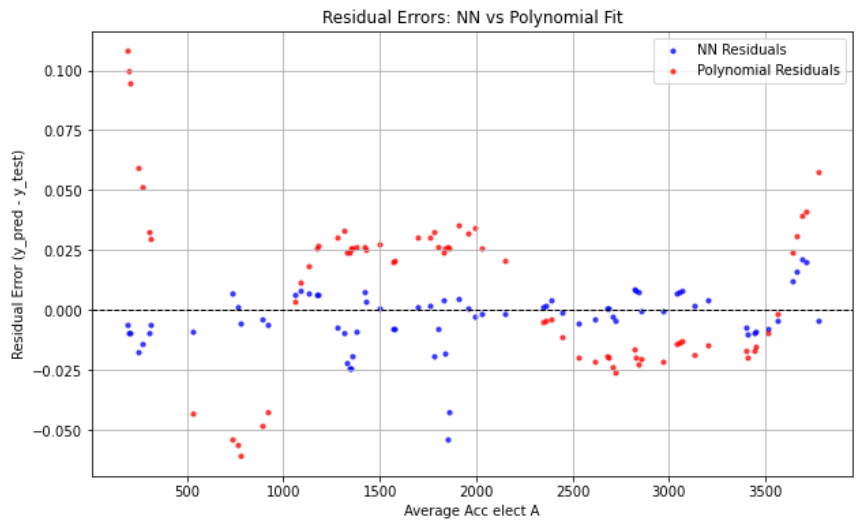
\includegraphics[width=0.75\linewidth]{graphics/hiradmat_SI.png}
    \caption{Residuals for the calibration curve of an ALPS Beam Position Monitor, based on the response of a single electrode.  (Courtesy of V. Stergiou and A. Boccardi, CERN).}
    \label{fig:wp3-hrm-si}
\end{figure}

The objective is to define and validate the algorithm for use within EURO-LABS. The implementation is planned to start in 2029, after the CERN long shutdown (2026-2029). This timeline provides sufficient time for the prototyping and testing of new electronic components, with the new system becoming operational after the restart.

\subparagraph{Task 3.2 : Technology Infrastructures} \mbox{}

This task includes six specialized facilities focused on accelerator component R\&D also connected to the AMICI~\footnote{\url{https://amici.ijclab.in2p3.fr/}} collaboration. The facilities remain in close contact with ongoing R\&D initiatives in EUROPE as the I.FAST project~\footnote{\url{https://ifast-project.eut}} but also world-wide as PIP-II~\footnote{\url{https://pip2.fnal.gov}}, where demand for tests of magnets and superconducting cavities could arise, in an effort to attract users. However already observed in P1, only three of these facilities have so far been able to support TA projects and deliver Access Units (AUs).

Technical works or upgrades initiated by the facilities' management to support long-term service contracts with large projects have reduced the availability of certain infrastructures for individual TA projects eligible for EURO-LABS funding. This is particularly the case for the INFN LASA and THOR facilities, as explained in more detail below. Additionally, the unexpected loss of local technical expertise, combined with difficulties in assigning replacements, has blocked the UU-FREIA facility from continuing to provide TA, despite its promising start during P1.

During the 18 months of P2, a total of 744 AUs were delivered, mainly through remote access, bringing the cumulative total since the beginning of EURO-LABS to 1,236 AUs. This corresponds to 30\% of the planned AUs if only considering operational facilities, or 10\% when considering all six facilities as initially foreseen in the Grant Agreement.

The WP and Task Leaders are closely monitoring the situation. There is optimism that, with the completion of technical works in 2025, some facilities will be able to resume the delivery of TA projects, with discussions already underway. In parallel, a mitigation plan has been prepared, which foresees a reshuffling of resources within the Task, and, if necessary, at the WP level.

Details per facility are provided in the following paragraphs.

% \todo{Briefly explain the progress of the task in context to the DoA.}

\subsubsection*{Main Results and Achievements}

% \todo{Briefly summarise the main results and achievements of the WP in context of the DoA.}

\subparagraph{UU-FREIA}

FREIA had a spectacular startup during P1, delivering 50\% of the AUs promised in the Grant Agreement. However, during P2, FREIA has not provided any transnational access (TA). Although there were preliminary discussions about testing a PIP-II cavity, unfortunately no follow-up actions materialized.

A key limiting factor is the facility’s availability for small, short-term TA projects, given its current engagement in large-scale, long-term contracts for series testing of production modules destined for major future accelerator installations in Europe. This series testing significantly restricts the use of the liquefier, a critical component for carrying out short-term experimental work. In addition, the facility experienced the departure of a key mechanical engineer — an expert in cryogenics with deep knowledge of the installation — without a rapid replacement, further complicating the planning of future tests.
Nevertheless, all efforts will continue to be made to support any future TA requests should they arise.


\todo{I am waiting a summary fro Rocio on the status of the service improvements}

%To answer your questions/s: yes, they are interested in using our facility and will sign the document (it’s already done by our side), but you know how it is with especially MYRRHA, we are requested to not give any information (let it be slides, or just in a general chat) if it has not been previously approved by them. And even more without a signed contract…So unfortunately this is not just because we do not have yet have a signed contract, this will always be the case: they being mention in any way in future slides will need to be sent for their approval.
 

% I write you because we are in initial discussions with FNAL about the possibility of testing a PIPII cavity in Gersemi, and I have a question that I forgot the answer to after the SAM…Provided the TA is granted by the committee, the total amount of units that FREIA can provide, is it the 20\% of the total? For example, FREIA has a total of 960 TA units, could we then only provide max 192 TA units for this test? So could they then pay the rest of the amount themselves if needed?

% Since we do not know how is it going to look in the future for us (since we will have the liquefier kind of blocked by Minerva testing, with some small slots here and there, maybe) we would like to have this test done and accounted, even though it is not from an European Institution.

\subparagraph{INFN-LASA} 

LASA (Laboratory for Accelerators and Applied Superconductivity) hosts four test facilities dedicated to: superconducting (SC) magnets, superconducting (SC) RF cavities, high-brightness photocathodes for electron sources, and laser applications to high-power Fabry–Perot cavities and advanced timing systems. These facilities were initially conceived to support LASA’s internal research activities.

So far, LASA has not been able to accept any transnational access (TA) projects. The transition of these facilities towards external user access progressed more slowly than initially anticipated during 2023, due to two main factors. First, a significant portion of the researchers and the already limited technical support staff were heavily involved in planning the expansion of LASA’s infrastructure, which is set to double the laboratory’s surface area. Second, the gradual conversion and upgrading of critical infrastructures — including electrical systems and the cooling systems for cavities and magnets — toward the new layout and future installations blocked the availability for external users.

According to the current planning, these upgrade activities of LASA are expected to be completed in 2025. If this timeline is met, it would leave sufficient time to consider few TA requests until the project ends in 2026 from the pool of users who had already expressed interest in 2023, assuming their interest remains active.

% LASA (Laboratory for Accelerators and Applied Superconductivity) is characterized by the presence of four test facilities devoted to: Superconducting (SC) Magnets, Superconducting (SC) RF Cavities, High Brightness Photocathodes for Electron Sources and Laser Applications to High Power Fabry Perot Cavities and Advanced Timing Systems. The four facilities have been conceived as facilities to support the research activities undergoing at LASA.

%So far LASA was not able to accept any TA project. This because the activities relating to a transition of these facilities towards use by external users slowed down during 2023 compared to the initial expectations for two reasons: first, the commitment of a relevant part of the researchers involved and of the technical support (the latter already quite limited) of the laboratory in relation to the planning of the expansion of the LASA (by a factor equal to approximately 100\% of the surface), and second the gradual conversion of the current infrastructures relating to the electrical systems and the cavity and magnet cooling system towards the new layout and future installations.

% In the present planning these activities should be completed in 2025, which if indeed the case, leaves time to consider TA requests among the few who expressed interest already in 2023, should their interest remains. 

% Once these activities have been completed, we are now able to prepare the forwarding of requests discussed and received in the meantime in relation to some specific activities.
%Of course due to the specific period of the year we have to discuss the confirmation for these previous requests. 

%Superconducting cavities: we discussed a request from researchers from DESY and CEA for the test of a prototype SC RF cavity for the PIP II project. The test will last a week considering 3 days for cooling down and one for warming up. The measurement process will last 2 days (for a total of nearly 12 hours/each day to save on liquid helium). Looking at the relatively short time dedicated to the measurements we are evaluating the possibility to operate in a remote fashion.
%The same opportunity for a separate test with longer measurements time involved will be used by a researcher from JLab to learn as much as possible on handling SC RF cavities for an ERL Linac of mutual interest. For this request we have to consider also some issue related to the availability of the requested volume of liquid helium (1500 liters) with so a short forewarning.

%Laser applications: a request has been discussed about a user from IJCLab and University of Orsay to carry out measurements on the laser system available at LASA for photocathode and Fabry Perot cavity. He plans to stay here a week (5 days) working 8-10 hours every day. This would be the first activity of a longer usage of our facility.

%High Brightness Photocathodes: a request has been recently issued to make some tests on a HV DC test stand related to the development of a DC Gun to investigate the behavior of specific materials handling High Voltage. The request come from the University of Uppsala. This request would be the first of a few, involving also tests with materials at cryogenic temperature.


\subparagraph{INFN-THOR}

The THOR (Test in Horizontal) facility in Salerno is focused on superconducting magnet systems testing. Equipped with advanced cryogenic, vacuum, and electrical testing setups, the facility ensures high-quality assessments of critical technologies in the field of superconductivity. 

However up to June 2024 the Facility was fully engaged in supporting the development and testing of accelerator components, particularly for the GSI/FAIR project. Specifically, a series of tests on the SIS100 quadrupole doublet modules for the test facility FAIR have been performed for the final acceptance before their installation in the SIS100 tunnel now under construction in Darmstadt. Given the tight timeline of the test plan, the allocated time for Transnational Access (TA) was so far limited. This constraint was primarily due to the high-priority testing schedule, which required significant resources and time allocation.

Starting from July 2024, access to the THOR facility has been restricted due to an ongoing upgrade and consolidation. This upgrade aims to enhance the facility’s capabilities, improving efficiency and increasing the throughput of testing activities. Consequently, no external access could be scheduled during this period and until February 2025.

By March 2025, the commissioning of a fully equipped test facility will start, providing testing opportunities for TA users in the field of cryogenic, vacuum, electronics. However the continous engagement of the Facility management to support the GSI/FAIR project as high-priority poses potential constraints on planning TA access. All efforts will be made to accommodate possible external access slots, should the interest arises. 

\subparagraph{SUPRATECH}

The facility is actively participating in the PIP-II project of FermiLab in USA achieving through RAs to perform the tests and full validation of SC cavities designed within the project. The SUPRATECH maintains strong links with the CEA/LRFU Sygergium facilities, offering combined tests of accelerator components for full validation. 

Among its users, SUPRATECH is actively involved in the PIP-II project at Fermilab in the USA, performing tests and full validation of superconducting (SC) cavities designed for the project. SUPRATECH maintains strong collaborative ties with the CEA/LRFU Sygergium facilities, offering combined testing of accelerator components to ensure full validation.

% Three projects during the reference period. 

%For Zanon company (Italy) : Testing at cryogenic temperature of 3 prototypes Spoke resonator (SSR2) for PIP2 project
%All three cavities tested and shipped to Fermilab
%2 cavities have been validated and reached PIP-II project specifications
%1 not validated but shipped to Fermilab for R\&D tests
%Testing report issued to Zanon company.
%For Fermilab (USA) : 2 cryogenic tests of 1 prototype Spoke resonator (SSR1) before/after plasma processing.
%Under validation by USP

\subparagraph{CEA-IRFU/Synergium}

The CEA-IRFU Synergium hosts two platforms: \textbf{MACHAFILM} and \textbf{CRYOMECH}, specialized on material science at cryogenic temperatures. The Synergium cryogenic laboratories are involved in several European accelerator projects on superconducting RF (SRF) and magnet technology with strong collaborative ties with major institutes in Europe: CERN, INFN, STFC, HZB, CNRS, and world-wide: FNAL and JLAB. Through these links MACHAFILM platform have performed well supporting thre TA projects for remote access, delivering 70\% of the AU promised in the GA.

\subparagraph{XBOX}

The XBOX facility hosts klystron-based X-band test stands located at CERN. These test stands are dedicated to the testing and development of high-gradient accelerating structures and high-power RF components, initially developed for the CLIC project, but also applicable to R\&D for X-band FELs, Compton/Thomson sources, and potential RF units for linear accelerators. As a result, XBOX offers unique, state-of-the-art yet highly specialized capabilities, which makes it challenging to meet a broader and more diverse needs of a wider external user community.
Despite sustained publicity efforts during the reference period, the XBOX facility did not attract any new transnational access (TA) projects. 

\subparagraph{Task 3.3 : Electron and Plasma Beams} \mbox{}

% \todo{Briefly explain the progress of the task in context to the DoA.}

This task includes six facilities located across three laboratories, offering access to electron or plasma beams.

A combination of technical, safety, and administrative issues has prevented three of the facilities from becoming operational and providing access units since the beginning of EURO-LABS. The fourth facility, is a state-of-the-art plasma beam installation, which is currently being upgraded, thus not yet easily accessible to external users. The remaining two facilities were fully active in P2 and have performed exceptionally well, delivering 65\% more AUs than expected for the 18-month period of P2, raising the cumulative total to 1490 AUs since the start of the project. This figure for the two facilities, represents 34\% more AUs than originally promised at this stage, demonstrating their strong potential to absorb additional TA requests and potentially compensate for the lack of access at other facilities.

Beyond the TA projects, good progress has also been made on the Service Improvements, with the projects entering their implementation phase as planned.

Details for each facility are provided in the following paragraphs

\subsubsection*{Main Results and Achievements}

%\todo{Briefly summarise the main results and achievements of the WP in context of the DoA.}

\subparagraph{INFN-LNF}

The Frascati National Labs (LNF) of the Italian Institute for Nuclear Physics (INFN) offers TA through 2 facilities: BTF (Beam Test Facility) and SPARCLAB (Sources for Plasma Accelerators and Radiation Compton with Laser And Beam).

BTF is an infrastructure mainly dedicated to the development and testing of particle detectors, providing primary, fixed energy beam and secondary electron or positron beams with continuously tunable energy from \SI{30}{\MeV} to \SI{780}{\MeV} and multiplicity from $10^{10}$ particles/pulse down to a single particle/pulse in a Poisson stochastic regime.
SPARCLAB is a research infrastructure based on the combination of the high-brightness SPARC photo injector, providing electron beam at energies up to \SI{180}{\MeV}, with the high intensity FLAME laser, able to generate infrared laser pulses with $10^{19}$~W/cm$^2$ intensity. The facility is generally devoted to the R\&D on novel acceleration techniques, advanced diagnostics and generation of radiation ranging from THz to extreme UV light. 

In the reporting period both facilities have been in operation apart from some maintenance periods and, mostly for SPARCLAB, upgrade and installation activities.

\begin{description}

\item[INFN-LNF/BTF]
The operation of BTF in the reporting period has been quite smooth and regular. According to its specific inclination, the facility run for a wide user community in terms of research fields and geographical distribution (national and international). In this context the implementation of the TA modality supported by EUROLABS resulted to be almost straightforward. In the reporting period the facility provided access to 3 EUROLABS supported experiments, for a total of 4 weeks of run delivering 672 AUs, corresponding to 57\% of the promised total in the GA. 

Highlights of the experiments in Section~\ref{sec:wp3_scientific_output}

\item[INFN-LNF/SPARCLAB]

The operation of SPARCLAB in the reporting period was limited because of a total of 6 months of shutdown necessary to install a consolidation/upgrade plan and for setting-up a new facility for FEL radiation production in the THz range, the SABINA project. This program was partially funded by the local Regional Government and its timeline was mandatory and could not be postponed. SPARCLAB is also the test-stand were the R\&D on plasma acceleration, which is the backbone of the laboratory flagship project EuPRAXIA, is being carried on with the highest priority. The combination of these 2 circumstances, i.e. the installation of the new facility and the high priority assigned to internal scientific program during the operation period, left essentially no-space to accommodate slots for TA. As a consequence, no TA have been provided by SPARCLAB in the reporting period.
\end{description}

% \separatorline{0.3em}{0.5\textwidth}{0.4pt}

\subparagraph{KIT-ANKA} \mbox{}

\todo{add few intro lines here}
\begin{description}
  
\item[KIT-FLUTE] FLUTE delivered so far no TA experiment, however several important and fundamental improvements have been made to this accelerator test facility. During the evaluation of the EURO-LABS TA proposal preparatory FLUTE experiments showed that the shot-to-shot stability, especially the pointing stability, was not sufficient for more advanced experiments. We traced this back to the low stability of the aging RF system. KIT therefore decided to completely refurbish the entire RF system. We installed a new photoinjector electron source from RadiaBeam, a new linear accelerator (linac) module from Research Instruments. We also used this occasion to install two separate RF sources and amplifiers from ScandiNova for the photoinjector and for the linac module. This renewal now allows a more precise and, above all, independent setting of parameters (energy, phase) for the photoinjector and the linac, respectively. Furthermore, we replaced the photoinjector laser system with a new and more powerful one permitting a wider range of experiments like, for instance, FLUTE experiments with split-ring resonators, that were requested by users in the past for Transnational Access.

These necessary refurbishments of almost all fundamental components of the accelerator led unfortunately to some delays for restarting FLUTE. This was mostly due to problems with the two new klystrons, requiring several service visits by the manufacturer. After solving these issues, we could show during commissioning of the new RF system an improved stability by a factor of 10.

After finalizing the commissioning of the linac and the bunch compressor, as well as the associated diagnostics sections with the new RF system, we are now ready to perform first TA experiments with the completely refurbished accelerator. 
Spring 2026 we will have to dismantle FLUTE temporarily as scheduled to be able to install the novel cSTART test accelerator facility at KIT, a new storage ring in the FLUTE experimental hall. This new installation will also include a laser plasma accelerator. In parallel FLUTE will be installed again and connected to the cSTART ring, where FLUTE serves as an injector to cSTART or an independent test facility.

\item[KIT-KARA]

KARA provided TA for 5 experiments during the reference period, delivering 598 AUs, which combined the the AUs offered in P1 make the total 818 AUs corresponding to 93\% of the total promised at the GA. 

Highlights of the experiments in Section~\ref{sec:wp3_scientific_output}
\end{description}

On the \textbf{Service Improvements:}

\underline{\em{Simulation and Measurement Framework activities}}:  
The frame work online optics simulation in ocelot was extended by scripts to measure automated different accelerator parameters like chromaticity, dispersion, beta function and response matrix. Further tools for different beam bases alignment  techniques are currently in development together with one TA activity. Another class of measurements are camera image processing. There different open source tools and analysis frameworks have been evaluated. It was decided to use the area Detecot {Ref: \url{https://areadetector.github.io/areaDetector/index.html} for this application which is currently implemented at KARA and FLUTE. KIT also joined the python accelerator middle layer activities (Ref:\url{https://github.com/python-accelerator-middle-layer}) to benefit from the shared effort. The next step is to contribute to the code development and deployment of the system at KARA and FLUTE.

\underline{\em{Data Management Framework Activities}}: 
In-depth analysis and comparison of three research data management platforms: B2Share~\footnote{https://b2share.eudat.eu/}, RADAR~\footnote{https://radar.products.fiz-karlsruhe.de/en}, and Kadi4Mat~\footnote{https://kadi.iam.kit.edu/}. This evaluation aimed to select suitable tools for managing experimental physics data effectively. Each platform was assessed based on its capabilities for data storage, accessibility, and metadata handling. Special attention was given to the ability to structure and retrieve metadata efficiently. Analyzing different experiments revealed that the metadata must be identified at an individual measurement level. This ensures precise documentation and supports reproducibility in research workflows. A flexible metadata generation schema is under preparation to accommodate diverse experimental requirements. The evaluation also considered automation possibilities to reduce manual metadata entry. Security, scalability, and integration with existing infrastructure were additional factors in the assessment. The final selection will balance usability and long-term sustainability for research environments.

Next steps: Based on the gained experience, select the most suitable tool and implement the Data Handling Framework and metadata generation. Validate the chosen solution in real-world scenarios and refine the approach based on feedback.

% \separatorline{0.3em}{0.5\textwidth}{0.4pt}

\subparagraph{CLARA}
 
During the reporting period, the CLARA facility has continued its reconfiguration to enable operation at \SI{250}{MeV}. 
In parallel, the full energy beam exploitation (FEBE) experimental hutch has been assembled and major sub-assemblies such as the user experiment chambers, magnetics and light boxes have been installed. The FEBE Ti:sapphire laser system has also been commissioned, allowing the synchronised interaction of electron bunches with an approximate \SI{100}{TW} laser. 

As of March 2025, the CLARA build phase is complete and the electron gun has been successfully tested. Due to the extensive redevelopment of CLARA and delays to the operational reinstatement of the facility, the facility has not delivered any TA projects during the period. However, sub-system recommissioning and beam threading will continue through summer 2025 and it is anticipated that user beam access, including TA projects, will restart in Q3/Q4 2025.

% \separatorline{0.3em}{0.5\textwidth}{0.4pt}

\subparagraph{LPA UHI100 (CEA-LIDYL} 

No beamtime was delivered during P2 (and similarly during P1) due to delays caused by the French Nuclear Safety Authority (ASN) in granting a license for operating the facility. We are still awaiting the final operating license from ASN/CEA.

The entire experimental setup, including the laser and experimental equipment, was relocated from the main CEA site at Saclay to a satellite facility at Orme des Merisiers, just a few kilometers away. In order to begin full laser energy operations and deliver the laser-driven electron source, we were required to obtain a license from ASN (Nuclear Safety Authority). A temporary license was issued at the beginning of 2024, valid through the end of August 2024, which limited the generating conditions to a maximum electron energy of \SI{50}{MeV}, a repetition rate of one shot per minute, and a maximum charge of \SI{15}{\pico C/bunch}, thus resulting in degraded operating conditions.

A visit by ASN was scheduled on July 3rd, 2024, to assess the operating conditions of the laboratory. Based on the feedback received during the visit, modifications were suggested, and a revised request for experimental parameters aligned with our scientific program (higher energy, repetition rate, and charge in the electron beams) was submitted.

At the end of December 2024, ASN granted CEA a temporary license for communication with our team scheduled on January 13th, 2025. This license is valid for one year and permits parameters of 200 MeV, a maximum repetition rate of \SI{0.3}{Hz}, and a maximum charge of \SI{300}{\pico C/bunch}.

Before proceeding with full-power operations on target, we need to conduct test experiments to verify the deposited dose by the electrons and check the consistency of simulations with the experiments. These tests are planned for March 2025, and if all conditions are met and consistent, we should be able to move forward with full-power operations on target.

\todo{Text to include here from Sandrine on Service Improvement}

\subparagraph{Task 3.4 : Applications} \mbox{}

% \todo{Briefly explain the progress of the task in context to the DoA.}

This task includes two facilities: the {\bf INCT/RAPID} and the {\bf CERN/CLEAR}. During the reference period both facilities were able to provide 11 TA projects, delivering 385 AUs raising the total to 643 AUs corresponding to 36\% of the promised AUs in the GA. 

Details are briefly described below. 

\subsubsection*{Main Results and Achievements}

% \todo{Briefly summarise the main results and achievements of the WP in context of the DoA.}

\subparagraph*{INCT/RAPID} 
During P2, the INCT/RAPID facility provided access with EURO-LABS support, conducting seven projects (one of which is still ongoing) delivering 105 AUs. The experiments utilized the following instruments:
\begin{itemize}
\item LAE 10 accelerator with nanosecond pulse radiolysis setup – used to investigate basic mechanisms of ionizing radiation interactions in biological systems.
\item Electronica accelerator, generating a beam of electrons with an energy of 10 MeV – for sterilization and materials modification.
\item ILU 6 accelerator, utilizing an electron beam with energies of 1.7 MeV and < 300 keV – for controlled depth of electron range in treated products.
\end{itemize}
For the experiments carried out at the RAPID infrastructure, dosimetry measurements were performed by the INCT Laboratory of Technological Dose Measurements to ensure precise and accurate dose delivery to the treated samples. Additionally, other INCT infrastructure, such as Electron Paramagnetic Spectroscopy, was used to help characterize radiation-induced effects in materials.

The experiments focused on the application of electron beams to investigate the mechanisms of radical interactions, radiation-induced effects in materials, and the effects of electron beam irradiation on food and food ingredients. In the upcoming year, plans are in place to adjust the experimental setup for irradiation in the gaseous phase, in response to newly received project requests. This modification will broaden the scope of research conducted at INCT within the EURO-LABS framework.

Highlights of the TA experiments are listed in Section~\ref{sec:wp3_scientific_output}

% \separatorline{0.3em}{0.5\textwidth}{0.4pt}

\subparagraph*{CERN-CLEAR Facility}

CLEAR was fully operational during the reference period able to provide TA to four experiments delivering 280 AUs, which cumulative to those delivered in P1 raise to a total of 448 AUs correspond to 37\% of the total promised at the GA. 
The facility is heavily used for conducting research on future electron accelerators, in parallel to a rigorous research program on FLASH radiotherapy. 

Highlights of the TA experiments are listed in Section~\ref{sec:wp3_scientific_output}

On the \textbf{Service Improvements:}
The CLEAR planned service improvements are meant to improve the quality of the measurements and of the data acquisition process in areas critical for a large part of the users and increase the number of users that can access the facility per unit time. 
\begin{figure}[H]
    \centering
    % 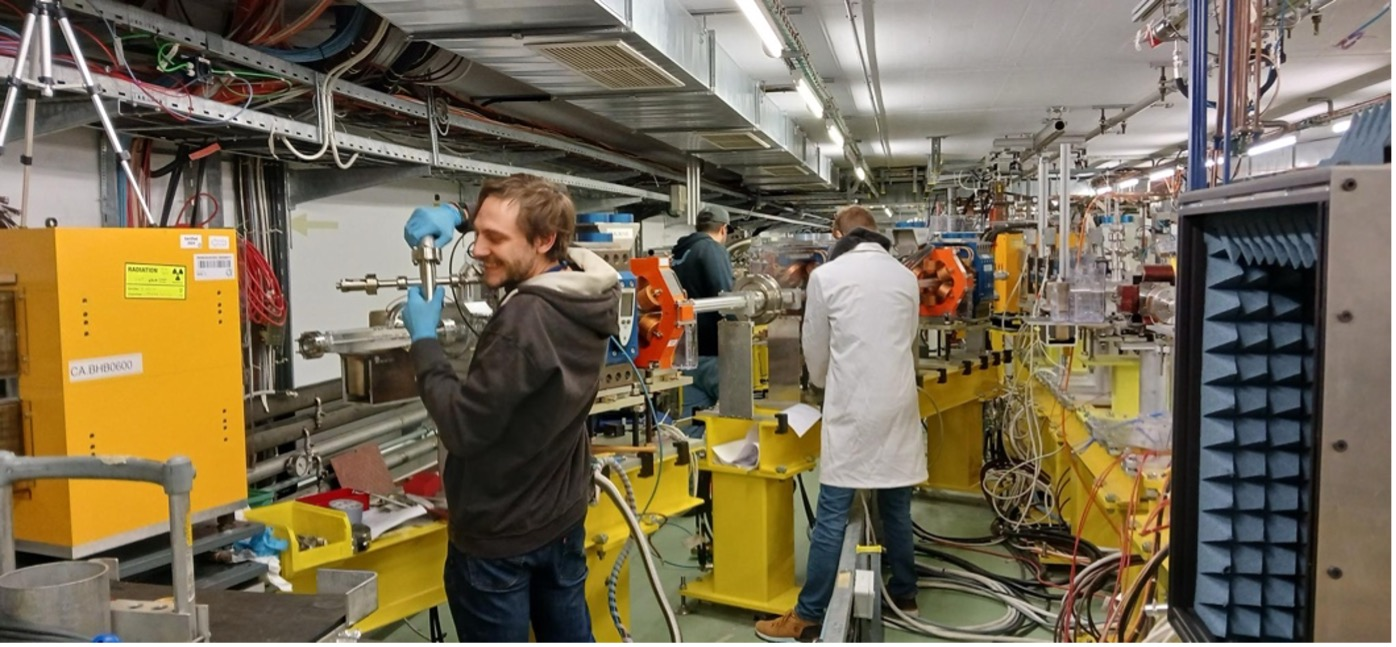
\includegraphics[width=0.78\linewidth]{graphics/CLEAR-2ndBLinstallation.jpg} \\
    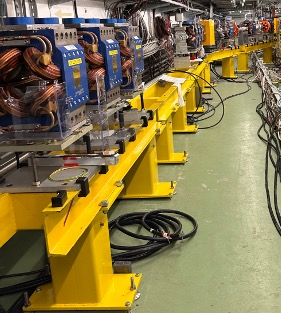
\includegraphics[width=0.60\linewidth]{graphics/CLEAR-2ndBLJan25.jpg}
    \caption{%Top: photo during the installation of the new beam line in the CLEAR facility.
    Photo of the new beam line of the CLEAR facility at the end of installation activities in January 2025.}
    \label{fig:wp3-clear-2ndbl-inst}
\end{figure}

The main CLEAR service improvement consist in the construction of a new beam line. This line will allow a faster turn-around of experiment, minimizing installation time, and will provide an end-of-line experimental station with added beam flexibility and improved handling/measurement hardware. The activity has been fully approved by CERN management in June 2023 and the beam line design was completed at beginning 2024. Most of hardware is being re-used from the previous CTF3 installation. Most components of the beam line have been installed in the winter shut-down 2024-2025 (see Figure~\ref{fig:wp3-clear-2ndbl-inst}).

The completion of the installation and its initial commissioning is planned for August-September 2025. Although mainly funded by CERN/CLEAR budget (total estimated cost ~ 180 kCHF), several items, in particular ones relevant for the end-of-line experimental area, have been purchased using EURO-LABS funding. These includes a beam current measurement device (ICT), an optical table, vacuum and optical components, beam screens and associated cameras, plus drawing office work. A new version of the handling C-robot was also designed, built and tested. Additional items still to be purchased using EURO-LABS funds are 1) an ionization chamber for real-time dosimetry, 2) two vacuum chambers for the two new beam line dipoles, 3) some ADC and timing modules and other acquisition and data handling hardware.
%\begin{figure}[H]
%    \centering
%    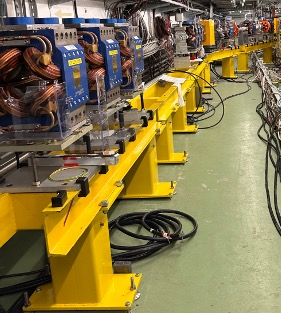
\includegraphics[width=0.78\linewidth]{graphics/CLEAR-2ndBLJan25.jpg}
%    \caption{Photo of the new beam line of the CLEAR facility at the end of January 2025.}
%    \label{fig:wp3-clear-2ndbl}
%\end{figure}

\todo{Add a paragraph to emphasize CLEAR's contribution to ATSOA24 and expected ATSOA25}


\subsubsection*{Deviations and Corrective Actions}
\label{sec:wp3_deviations}
% \todo{Briefly summarize any deviations and performed corrective actions of the WP in context of the DoA.}

The WP3 facilities are currently lagging behind in providing the required number of TA projects and Access Units (AUs). By the end of P2, the facilities have collectively delivered only 26\% of the promised TA projects and 35\% of the planned AUs. However, behind this overall picture, there are significant variations between individual facilities as explained above.

To address these deviations, we will continue to closely monitor the situation and propose adjustments to the allocation of project resources. Priority will be given to reallocating resources towards higher-performing facilities, first within the Task and, if necessary, across the entire Work Package. This strategy aims to maximize the overall TA delivery by supporting additional projects at facilities with greater TA capacity.

Based on present performance and future expectations we can classify the facilities as follows:
\begin{description}
    \item[Overperforming:] HiRadMAt, KIT/KARA. \\
        Performing very well. Could absorb additional TA projects if needed.
    \item[Within expectations:] LRFU-Synergium, IJCLAB-SUPRATECH, CEA-LPA-UHI100, STFC-CLARA, INFN-BTF, INCT-RAPID \\
        Maintaining expected performance levels. Expected to deliver according to the original schedule. 
    \item[Below expectations:] UU-FREIA, INF-LASA, INFN-THOR, XBOX, KIT/FLUTE, INFN-SPARCLAB, CLEAR. \\
        Facing technical or administrative delays. Unlikely to fully deliver the planned TAs. Accepted to release TA resources.
\end{description}
Further details provided for selected facilities in the following paragraphs.

% Table~\ref{tabl:wp3-deviations} summarizes the current status, with further details provided for selected facilities in the following sections.
%\begin{table}[H]
%    \centering
%    \begin{tabularx}{\textwidth}{|c|X|} \hline
%    \rowcolor{lightgray}
%    \textbf{Facility} & \textbf{Comments} \\ \hline
%    \multicolumn{2}{|c|}{\textbf{Overperforming}} \\ \hline
%    HiRadMat & \multirow{2}{\hsize}{Performing very well. Could absorb additional TA projects if needed.} \\ 
%    KIT/KARA & \\ \hline
%   \multicolumn{2}{|c|}{\textbf{Within expectations}} \\ \hline
%    LRFU-Synergium & \multirow{6}{\hsize}{Expected to deliver according to the original schedule. Maintaining expected performance levels.} \\ 
%    CEA-LPA-UHI100 & \\ 
%    STFC-CLARA & \\
%    INFN-BTF & \\
%    IJClab-SUPRATECH & \\
%    INCT-RAPID & \\ \hline
    
%   \multicolumn{2}{|c|}{\textbf{Below expectations}} \\ \hline
%   UU-FREIA & \multirow{6}{\hsize}{Facing technical or administrative delays. Unlikely to fully deliver the planned TAs. Accepted to release TA resources.} \\ 
%   KIT-FLUTE & \\
%    XBOX & \\ 
%    INFN-LASA & \\
%    INFN-THOR & \\
%    INFN-SPARCLAB
%    CLEAR & \\ \hline
    
%    \end{tabularx}
%    \caption{Summary of WP3 facility status and group comments.}
%    \label{tabl:wp3-deviations}
%\end{table}

\paragraph{HiRadMat} HiRadMat has already used 82\% of its allocated 4800 Access Units (AUs) at the end of the second reference period. This high usage rate reflects the facility’s strong visibility, supported both by EURO-LABS dissemination efforts and the production of promotional videos. The remaining AUs are sufficient to cover part of the experiments planned for 2025; however, there will be no budget available to support the remaining 2025 experiments or those anticipated in 2026, the exact number of which is still uncertain.

HiRadMat would welcome additional funding to support continued transnational access, as well as user assistance with logistics and simulation efforts.

\paragraph{LPA UHI100 (CEA-LIDYL)} We have plan to deliver beamtime as much as we will be able to do. We have already a proposal from an Italian Team that should be submitted. The LPA-UHI100 facility team is considering the technical feasibility of the proposal with the applicants, before submission. And we are working on a 2nd proposal which could be the following of the 1st one, depending on the results obtained. We will keep advertising about the TNA through EUROLABS, participating to international/national conferences this year 2025.  We have already discussed with other communities and in particular physico –chemists and radiobiologists who want to use the extrem dose rate delivered by our laser-driven electron sources to test the response of biological material to such irradiations, in the context of FLASH radiotherapy, and to validate dosimeters developed for such high dose rate source.  

1 beam time project (160 hours) for 2025, in preparation for submission next march 2025, to test a temporal diagnostic adapted to the extremely short duration of the LPA electron beams. The beamtime could be allocated at the second semester of 2025.

We will try to deliver another beamtime period (160hours) in the first semester 2026, planning a maximum of 2 runs in 2026 (320hours max in 2026).

\paragraph{INFN-LNF/(BTF, SPARCLAB)}

The perspectives for the completion of the EURO-LABS TA program for BTF look quite secure. The facility staff is now systematically promoting the opportunity of supported TA to the reference community, with positive returns, and 4 out of 7 TA weeks planned for the whole project have been already delivered. The staff is confident that the remaining 3 will be assigned and delivered by the end of 2025, and some space will be available to eventually accommodate 2-3 extra weeks in the 2026 before the project conclusion.
For what concerns SPARCLAB the situation looks far less optimal. As mentioned, none of the 9 weeks of TA allocated in the project have been delivered so far, and it not realistic to think recovering all in the time left till the end of the project for the mentioned reasons. In 2025 the new facility EuAPS funded by the Next Generation EU program will be installed in the SPARCLAB bunker requiring a 4 months shutdown. In the present scenario the number of allocable TA weeks at SPARCLAB before the EURO-LABS project end in August 2026 is 2-3. The SPARCLAB staff is committed to promoting this opportunity to its international reference community.

\subsubsection*{Milestones and Deliverables}

%{\fontsize{9}{11}\selectfont
%\begin{center}
%  \begin{tabular}[t]{!{\color{mygray}\vrule}p{0.10\linewidth}!
%  {\color{mygray}\vrule}p{0.60\linewidth}!
%  {\color{mygray}\vrule}p{0.20\linewidth}!{\color{mygray}\vrule} } \hline
%    \rowcolor{mycyan} & {\bf Title} & {\bf Status} \\ \hline
%    \cellcolor{mycyan}{\bf D1.x}: &  &  \\ \hline
%  \end{tabular}
%\end{center}
%}

There were no Milestones nor Deliverables for WP3 for the reference period. 

\subsubsection*{Project Meetings}

\begin{table}[H]
    \centering
    \caption{Summary of WP3 meetings and discussed subjects.}
    \begin{tabularx}{\textwidth}{|c|c|X|} \hline
        \rowcolor{mycyan}
        \textbf{Date} & \textbf{Meeting} & \textbf{Subject} \\ \hline
        2023-09-11 & TL02 - Task Leader's meeting & Regular meeting - progress report \\ \hline
        2023-09-25 & WP3-03 Meeting & Regular WP meeting - progress report from the facilities \\ \hline
        2023-10-11 & Special meeting LASA-THOR & Discuss status and TA possibilities \\ \hline
        2024-01-25 & WP3-04 Meeting & Regular WP meeting - progress report from the facilities \\ \hline
        2024-09-06 & TL03 - Task Leader's meeting & Regular meeting - progress report \\ \hline
        2024-09-13 & WP3-05 Meeting & Regular WP meeting - progress report from the facilities \\ \hline
        2024-10-29 & WP3-06 Meeting & Regular WP meeting - progress report from the facilities \\ \hline
        2025-02-11 & TL04 - Task Leader's meeting & Regular meeting - progress report \\ \hline
    \end{tabularx}
    \label{tab:meetings}
\end{table}
Besides these remote zoom meetings, the two key WP3 meetigns were organized during the Annual Meetings of the Project, in Krakow in 2023 and at CERN in 2024, and several ad-hoc meetings with the facility coordinators and task leaders were organized via zoom, when it was necessary. 


%  {\color{mygray}\vrule}p{0.40\linewidth}!

%%%%%%%%%%%%%%%%%%%%%%%%%%%%%%%%%%%%%%%%%